\documentclass[tikz,border=8pt]{standalone}
\usepackage[T1]{fontenc}
\usepackage{lmodern}
\usepackage{amsmath}
\usetikzlibrary{arrows.meta,positioning,calc,fit,backgrounds}

\definecolor{navy}{HTML}{25364A}
\definecolor{blue}{HTML}{56B4E9}
\definecolor{orange}{HTML}{E69F00}
\definecolor{green}{HTML}{009E73}
\definecolor{purple}{HTML}{7B61A8}
\definecolor{lightblue}{HTML}{EAF5FB}
\definecolor{lightorange}{HTML}{FFF4DF}
\definecolor{lightgray}{HTML}{F3F4F6}
\definecolor{midgray}{HTML}{6B7280}

\tikzset{
  >={Latex[length=2.6mm]},
  flow/.style={->, very thick, draw=navy, rounded corners=3pt},
  optional/.style={->, thick, dashed, draw=midgray, rounded corners=3pt},
  data/.style={draw=#1, fill=#1!10, very thick, rounded corners=4pt,
               minimum width=38mm, minimum height=13mm, align=center,
               font=\rmfamily\bfseries},
  input/.style={draw=midgray, fill=lightgray, thick, rounded corners=3pt,
                minimum width=39mm, minimum height=11mm, align=center,
                font=\rmfamily\small},
  block/.style={draw=navy, fill=white, very thick, rounded corners=4pt,
                minimum width=43mm, minimum height=14mm, align=center,
                font=\rmfamily\bfseries},
  head/.style={draw=#1, fill=#1!12, very thick, rounded corners=4pt,
               minimum width=42mm, minimum height=14mm, align=center,
               font=\rmfamily\bfseries},
  output/.style={draw=#1, fill=white, thick, rounded corners=3pt,
                 minimum width=42mm, minimum height=12mm, align=center,
                 font=\rmfamily\small},
  loss/.style={draw=#1, fill=#1, text=white, very thick, rounded corners=4pt,
               minimum width=37mm, minimum height=12mm, align=center,
               font=\rmfamily\bfseries\fontsize{10.5}{12}\selectfont\boldmath},
  note/.style={font=\rmfamily\footnotesize, text=midgray, align=center}
}

\begin{document}
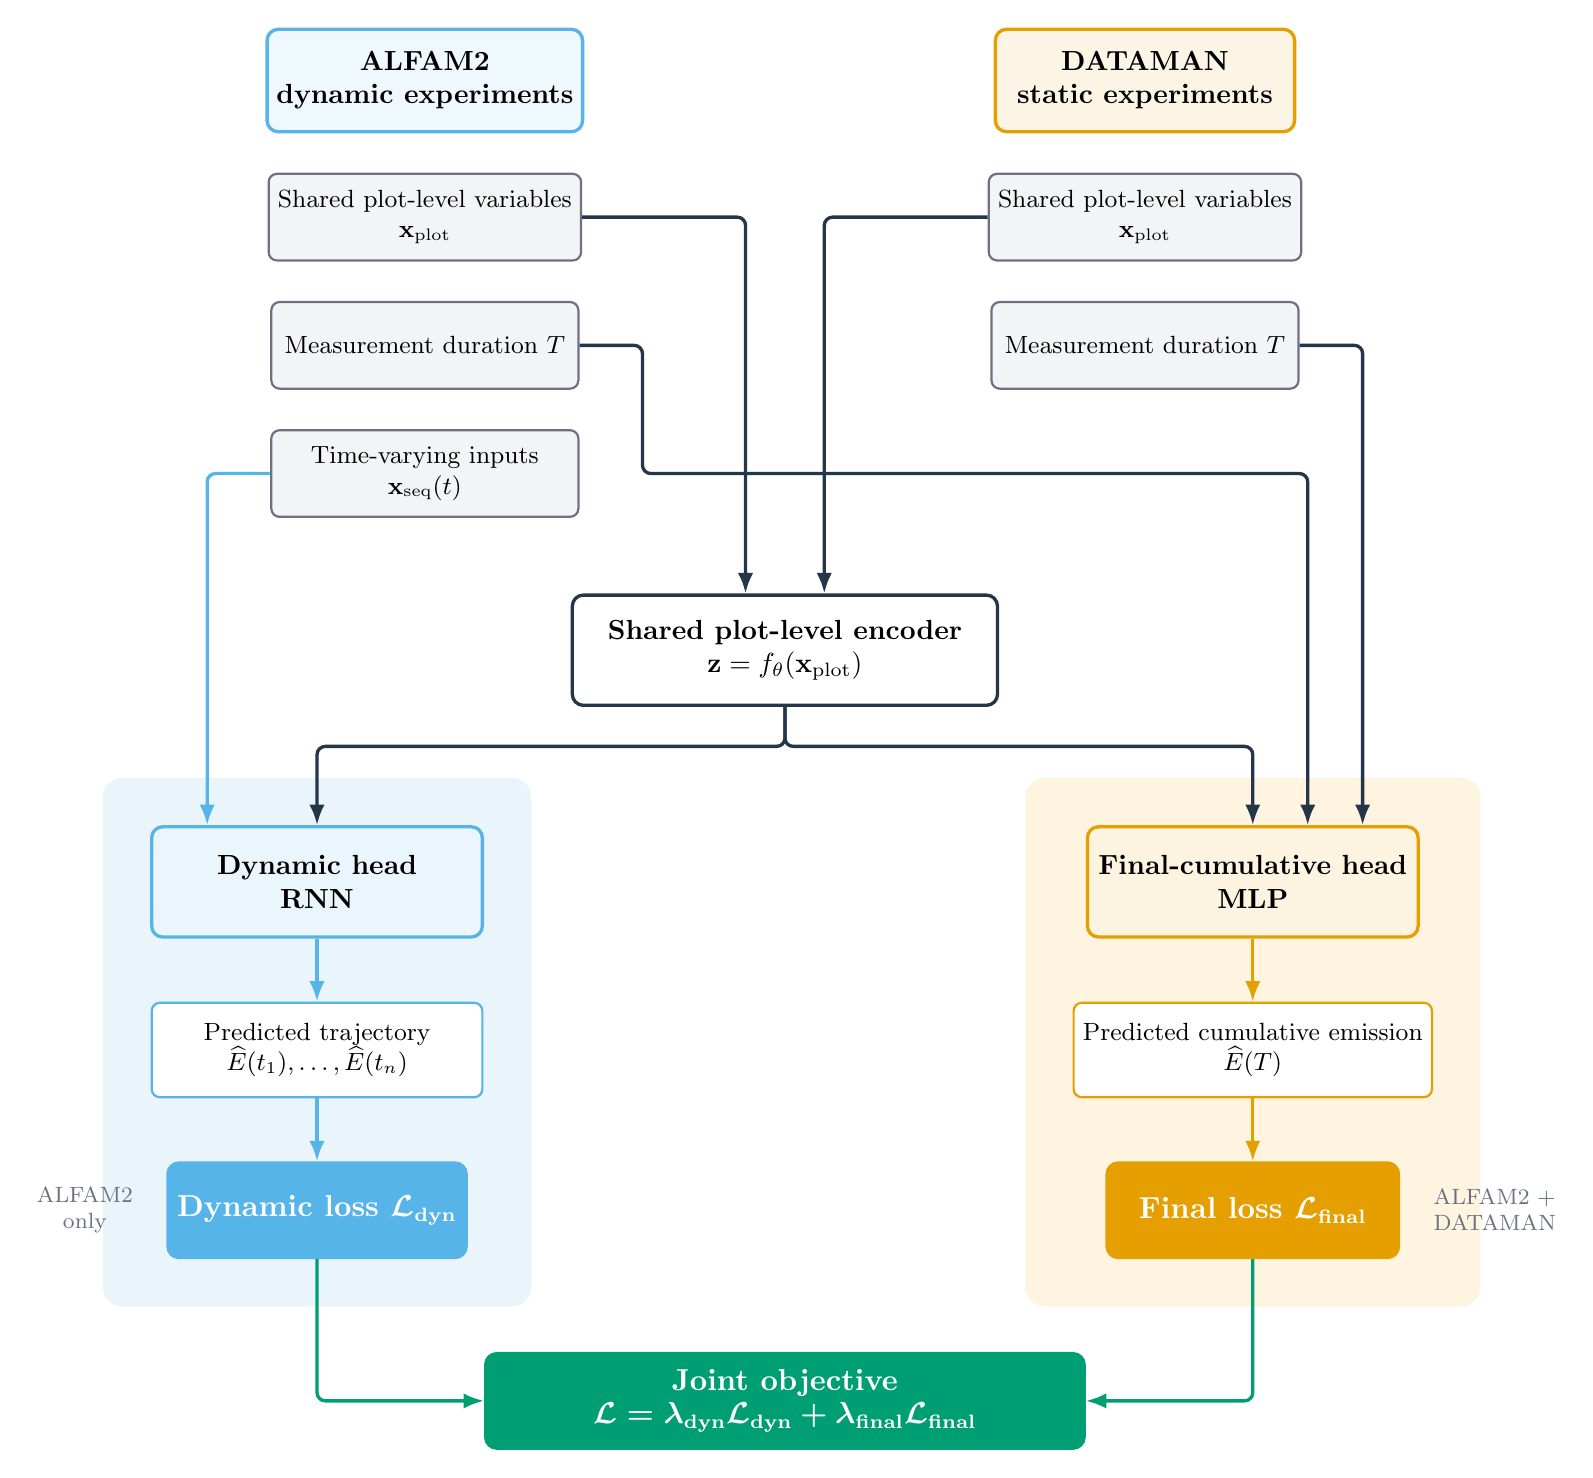
\begin{tikzpicture}[node distance=8mm and 15mm]

% Data sources and their available inputs
\node[data=blue] (alfam) {ALFAM2\\dynamic experiments};
\node[data=orange, right=52mm of alfam] (dataman) {DATAMAN\\static experiments};

\node[input, below=5mm of alfam] (alfamstatic)
  {Shared plot-level variables\\$\mathbf{x}_{\mathrm{plot}}$};
\node[input, below=5mm of dataman] (datastatic)
  {Shared plot-level variables\\$\mathbf{x}_{\mathrm{plot}}$};

\node[input, below=5mm of alfamstatic] (alfamduration)
  {Measurement duration $T$};
\node[input, below=5mm of alfamduration] (sequence)
  {Time-varying inputs\\$\mathbf{x}_{\mathrm{seq}}(t)$};
\node[input, below=5mm of datastatic] (duration)
  {Measurement duration $T$};

% Shared representation
\coordinate (encmid) at ($(alfamstatic)!0.5!(datastatic)+(0,-55mm)$);
\node[block, minimum width=54mm] (encoder) at (encmid)
  {Shared plot-level encoder\\$\mathbf{z}=f_{\theta}(\mathbf{x}_{\mathrm{plot}})$};

\draw[flow] (alfamstatic.east)
  -- ([xshift=-5mm]encoder.north |- alfamstatic.east)
  -- ([xshift=-5mm]encoder.north);
\draw[flow] (datastatic.west)
  -- ([xshift=5mm]encoder.north |- datastatic.west)
  -- ([xshift=5mm]encoder.north);

% Two task-specific heads
\node[head=blue, below left=15mm and 11mm of encoder] (dynhead)
  {Dynamic head\\RNN};
\node[head=orange, below right=15mm and 11mm of encoder] (finalhead)
  {Final-cumulative head\\MLP};

\draw[flow] (encoder.south) -- ++(0,-5mm) -| (dynhead.north);
\draw[flow] (encoder.south) -- ++(0,-5mm) -| (finalhead.north);
\coordinate (sequenceturn) at ([xshift=-8mm]sequence.west);
\draw[flow, draw=blue] (sequence.west)
  -- (sequenceturn)
  -- (sequenceturn |- dynhead.north);
\coordinate (durationturn) at ([xshift=8mm]duration.east);
\draw[flow] (duration.east)
  -- (durationturn)
  -- (durationturn |- finalhead.north);
\coordinate (alfamfinalentry) at
  ($(finalhead.north)!0.5!(durationturn |- finalhead.north)$);
\coordinate (alfamdurationexit) at ([xshift=8mm]alfamduration.east);
\coordinate (alfamdurationdown) at
  (sequence.center -| alfamdurationexit);
\coordinate (alfamdurationright) at
  (alfamfinalentry |- alfamdurationdown);
\draw[flow] (alfamduration.east)
  -- (alfamdurationexit)
  -- (alfamdurationdown)
  -- (alfamdurationright)
  -- (alfamfinalentry);

% Predictions and supervised losses
\node[output=blue, below=of dynhead] (dynout)
  {Predicted trajectory\\$\widehat{E}(t_1),\ldots,\widehat{E}(t_n)$};
\node[output=orange, below=of finalhead] (finalout)
  {Predicted cumulative emission\\$\widehat{E}(T)$};
\draw[flow, draw=blue] (dynhead) -- (dynout);
\draw[flow, draw=orange] (finalhead) -- (finalout);

\node[loss=blue, below=of dynout] (dynloss)
  {Dynamic loss $\boldsymbol{\mathcal{L}}_{\mathbf{dyn}}$};
\node[loss=orange, below=of finalout] (finalloss)
  {Final loss $\boldsymbol{\mathcal{L}}_{\mathbf{final}}$};
\draw[flow, draw=blue] (dynout) -- (dynloss);
\draw[flow, draw=orange] (finalout) -- (finalloss);

\node[note, left=3mm of dynloss] {ALFAM2\\only};
\node[note, right=3mm of finalloss] {ALFAM2 +\\DATAMAN};

% Joint objective
\node[loss=green, below=18mm of $(dynloss)!0.5!(finalloss)$,
      minimum width=76mm] (total)
  {Joint objective\\$\boldsymbol{\mathcal{L}}=\boldsymbol{\lambda}_{\mathbf{dyn}}\boldsymbol{\mathcal{L}}_{\mathbf{dyn}}
   +\boldsymbol{\lambda}_{\mathbf{final}}\boldsymbol{\mathcal{L}}_{\mathbf{final}}$};
\draw[flow, draw=green] (dynloss.south) |- (total.west);
\draw[flow, draw=green] (finalloss.south) |- (total.east);

% Background groups improve immediate reading of the two tasks.
\begin{scope}[on background layer]
  \node[fit=(dynhead)(dynout)(dynloss), fill=lightblue, rounded corners=7pt,
        inner sep=6mm] {};
  \node[fit=(finalhead)(finalout)(finalloss), fill=lightorange,
        rounded corners=7pt, inner sep=6mm] {};
\end{scope}

\end{tikzpicture}
\end{document}
